\documentclass[a4paper,11pt]{article}
\usepackage{graphicx}
\usepackage[utf8]{inputenc}  
\usepackage[T1]{fontenc}
\usepackage{gensymb}

\usepackage{helvet}%Police Arial
\renewcommand{\familydefault}{\sfdefault}

\usepackage[top = 1cm, bottom = 2cm, left = 1cm, right = 1cm]{geometry}
\usepackage{titlesec}
\setcounter{secnumdepth}{4}
\usepackage{xcolor}
\usepackage{amssymb} %double flèche de réaction
\usepackage{xtab}%tableau sur plusieurs pages
\usepackage{esvect}%grands vecteurs

 \usepackage[version=4]{mhchem} %equations chimiques

\usepackage{array}
\usepackage{chemfig}
\usepackage{multirow}
\usepackage{sectsty}
\usepackage{caption}
\usepackage{amsmath}
\usepackage{amssymb}
\usepackage[cal=boondoxo]{mathalfa} 
\usepackage{enumitem}
\usepackage{lastpage}
\usepackage{tcolorbox}
\usepackage{siunitx}
\usepackage{tikz}
\usetikzlibrary{calc}
\usepackage{multicol}
\usepackage{eqnarray}

 \sisetup{
    detect-all,
    output-decimal-marker={,},
    group-minimum-digits = 3,
    group-separator={~},
    number-unit-separator={~},
    inter-unit-product={~}
} %setup pour SIunitx

\usepackage{listings}%pour insérer le code python
\definecolor{codegreen}{rgb}{0,0.6,0}
\definecolor{codegray}{rgb}{0.5,0.5,0.5}
\definecolor{codepurple}{rgb}{0.58,0,0.82}
\definecolor{backcolour}{rgb}{0.95,0.95,0.92}

\graphicspath{ {/home/remy/Documents/Enseignement/2022/Tspe/C9/Ressources/} }

\sectionfont{\fontsize{14}{8}\selectfont}
\renewcommand{\thesection}{\arabic{section}.}
\renewcommand{\thesubsection}{\hspace{1cm}\alph{subsection}.}

\title{\vspace{-1cm}\large 
	\begin{tabular}{|>{\centering}m{5cm}|>{\centering}m{8cm}|>{\centering\arraybackslash}m{4cm}|}
	\hline
	DS 4 & \textbf{\textsc{Équilibres chimiques et Équilibres acide-base}} &  Chapitre 7 et 8\\
	\hline
	\end{tabular}}
\date{}

\newpagestyle{mystyle}{%
\setfoot{}{\thepage\,$|$\,\pageref{LastPage}}{}
}
\renewpagestyle{plain}{%
\setfoot{}{\thepage\,$|$\,\pageref{LastPage}}{}
}

\pagestyle{mystyle}

\newenvironment{itemize*}%
  {\begin{itemize}[label=$-$]%
    \setlength{\itemsep}{0pt}%
    \setlength{\parskip}{0pt}}%
  {\end{itemize}}

\newenvironment{itemize**}%
  {\begin{itemize}[label=]%
    \setlength{\itemsep}{0pt}%
    \setlength{\parskip}{0pt}}%
  {\end{itemize}}
  
\begin{document}
\maketitle
\vspace{-2cm}
Le sel d'oseil est une substance chimique présente osus forme d'un solide cristallin blanc, incolore et inodore. Il était historiquement extrait de certaines plantes telles que l'oseille ou la rhubarbe. On le nomme, en nomenclature officielle, l'acide éthendioïque ou plus communément acide oxalique. Cette substance est actuellement utilisée dans l'industrie pour la création de polymères mais peut être aussi employée dans de nombreux autres domaines : produits nettoyant, répulsif à frelon en apiculture, etc.\\
L'objectif de cet exercice est de valider deux hypothèses sur le type d'acidité de l'acide oxalique puis dans un second temps de retrouver la formulation de cet acide dans un produit ménager.
\section{Première hypothèse : l'acide oxalique est un diacide fort}
\textbf{Données :}
\begin{itemize}
    \item Tableau regroupant les électronégativités des atomes de carbone, d'oxygène et d'hydrogène :\\
    \begin{tabular}{|c|c|c|c|}
    \hline & Carbone & Oxygène & Hydrogène  \\
    \hline Électronégativité & 2,55 & 3,44 & 2,20\\
    \hline
    \end{tabular}
    \item Formule semi-développée de l'acide oxalique :\\
    \begin{center} \chemfig{HO-[::30]C(=[::120]O)-C(=[::30]O)-[::-30]OH}
    \end{center}
\end{itemize}
\begin{enumerate}
    \item Donner la définition d'une espèce acide selon Brönsted puis, justifier le terme diacide pour l'acide oxalique.
    \item Représenter sur votre copie la représentation de Lewis de l'acide oxalique ainsi que celle de l'une des deux autres formes acido-basiques. Justifier le caractère acide des atomes d'hydrogène dans la molécule.
    \item Donner les deux couples acide/base associés à l'acide oxalique puis donner la particularité de l'espèce chimique présente dans les deux couples.
\end{enumerate}
Au laboratoire, on mesure la valeur du pH d'une solution d'acide oxalique de concentration en acide apporté $C_0$ égale à \num{5,00e-2} \unit{\mole\per\liter}. La valeur du pH obtenu est de \num{1,47}.\\
On souhaite modéliser la transformation chimique entre l'acide oxalique et l'eau en émettant l'hypothèse que l'acide oxalique se comporte comme un diacide fort. On notera \ce{AH2 (aq)} l'acide oxalique et \ce{A^2- (aq)} l'ion oxalate.
\begin{enumerate}
\setcounter{enumi}{3}
    \item Écrire l'équation de la réaction modélisant cette transformation chimique.
    \item En déduire que, dans le cas de l'hypothèse précédente, la valeur de la concentration en quantité de matière en ions oxonium $[\ce{H3O+}]$ est égale à \num{1,00e-1} \unit{\mole\per\liter}. On pourra s'appuyer sur un tableau d'avancement.\\
    \textbf{Donnée :}\\
    La concentration standard $C^0$ est égale à 1,0 \unit{\mole\per\liter}.
    \item À l'aide su résultat précédent, calculer la valeur du pH théorique de la solution, puis justifier que l'hypothèse affirmant que l'acide oxalique est un diacide fort n'est pas valide.
\end{enumerate}

\section{Deuxième hypothèse : l'acide oxalique se comporte comme un monoacide faible en solution.}
\textbf{Données : }
\begin{itemize}
    \item La concentration en acide apporté $C_0$ de la solution d'acide oxalique est égale à \num{5,00e-2} \unit{\mole\per\liter}.
    \item Valeur du pKa de la première acidité : $pKa_1$ = 1,2.
    \item Équation de la réaction associée à la première acidité : \\
    \begin{center}
        \ce{AH2(aq) + H2O(l) <=> AH-(aq) + H3O+(aq)}
    \end{center}
    \item Rappel de la valeur expérimentale du pH de la solution d'acide oxalique : $pH_exp$ = 1,47.
\end{itemize}
\begin{enumerate}
    \item Écrire l'équation de la réaction modélisant  la transformation chimique de l'espèce \ce{AH-} avec l'eau, associée à la deuxième acidité.
    \item À l'aide de la figure 1, déterminer la valeur du pKa de la deuxième acidité de l'acide oxalique.
\end{enumerate}
\begin{figure}[h]
    \centering
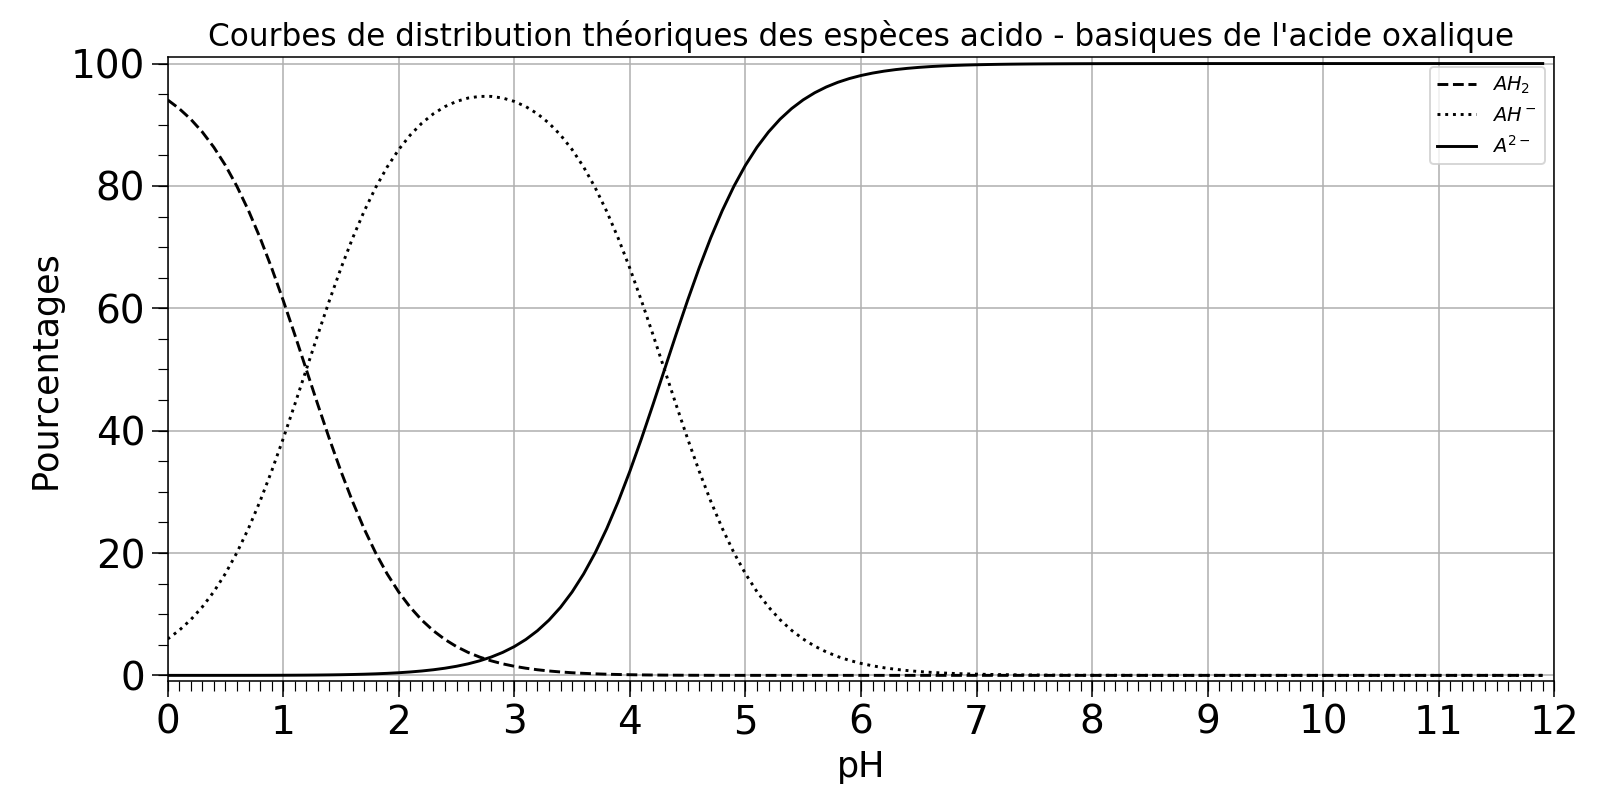
\includegraphics[scale=.3]{Ressources/TSPE_C8_Eval_Fig1.png}
    \caption{Diagramme théorique de distribution des différentes espèces acido-basiques de l'acide oxalique}
    \label{fig:my_label}
\end{figure}
\begin{enumerate}
\setcounter{enumi}{2}
    \item À l'aide de la figure 1 et de la valeur du pH de la solution, donner le pourcentage approximatif de chaque espèce présente dans la solution puis, justifier que l'on peut émettre l'hypothèse selon laquelle l'acide oxalique se comporte comme un monoacide.
\end{enumerate}
Dans le cadre de cette deuxième hypothèse, nous allons essayer de retrouver la valeur du pH théorique de la solution.
\begin{enumerate}
\setcounter{enumi}{3}
    \item À partir de l'équation de la réaction présentée en données, exprimer la constante d'acidité $Ka_1$ en fonction de la concentration des différentes espèces chimiques à l'équilibre.
    \item À l'aide de la question précédente, justifier que la concentration en ion oxonium à l'équilibre, notée $h$, vérifie l'équation du second degré suivante :
    \begin{eqnarray}
    h^2 + Ka_1 \cdot h - Ka_1 \cdot C_0 =0\nonumber
    \end{eqnarray}
\end{enumerate}
Pour retrouver la concentration en ions oxonium, nous utilisons un code python incomplet donné en figure 2 permettant de calculer directement la concentration $h$ en ions oxonium, ainsi que la valeur du pH théorique de la solution.
\begin{figure}
    \begin{minipage}{.1\linewidth} \hspace{.5cm} \end{minipage}
    \begin{minipage}{.8\linewidth}
    \textbf{Code python :}
    \begin{lstlisting}[showstringspaces=false,language = Python, numbers=left]
import math
pKa1 = float(input("pka1 du couple : "))
concentration=float(input("Concentration apportee en mol/L : ""))
Ka1 =
###Coefficients du polynome du deuxieme degre
a=1
b=Ka1
c=-Ka1*concentration
###Calcul du discriminant
Delta=b**2-4*a*c
##Solution pour [H3O+]
h=(-b +sqrt(Delta))/(2*a)
###pH final
pH = -math.log10(h)
###Ecrire des resultats
print('h=',format(h, "3.2E"),"mol/L",'  ',"pH final : ",round(pH,2))
\end{lstlisting}
\fbox{\textbf{Résultat du code : }h=3.29E-02 mol/L  pH final : 1.48}
\end{minipage}


    \caption{Code python permettant de calculer la concentration $h$ en ions oxonium et la valeur du pH théorique de la solution.}
    \label{fig:my_label}
\end{figure}
\begin{enumerate}
\setcounter{enumi}{5}
    \item Compléter la ligne 4 du code python par la formule permettant au programme de calculer la valeur de la constante d'acidité $Ka_1$.
    \item À l'aide du résultat calculé par python et des données, justifier le fait que l'acide oxalique se comporte bien comme un monoacide faible.
\end{enumerate}

\section{Formulation de l'acide oxalique}
Lors de l'achat de l'acide oxalique, on peut le trouver sous deux formes différentes. Dans un cas, il peut être pur et dans l'autre, il peut se trouver sous forme dihydratée. Un agent de laboratoire trouve un récipient contenant un solide blanc portant une étiquette avec la mention "acide oxalique" sans aucun autre précision.\\
Ne sachant pas si le produit est dihydraté ou non, il décide de faire un titrage par suivi pH-métrique d'une solution aqueuse de ce solide. Pour cela, il fabrique une solution connue par dissolution d'une masse d'acide oxalique $m$ = \num{0,27} \unit{\gram} avec une incertitude-type $u(m)$ = \num{0,01} \unit{\gram} dans une fiole jaugée de volume $V$ = \num{100,0} \unit{\milli\liter} avec une incertitude-type $u(V)$ = \num{0,1} \unit{\milli\liter}.\\
\textbf{Données :}
\begin{itemize}
    \item l'incertitude-type $u(X)$ sur une grandeur $X$ lorsqu'elle est obtenue à partir d'autres grandeurs indépendantes s'écrit pour une division :
    \begin{eqnarray}
        \text{Si } X=\dfrac{Y}{Z} \text{ alors } u(X) = x \cdot \sqrt{\left(\dfrac{u(Y)}{Y}\right)^2 + \left(\dfrac{u(Z)}{Z}\right)^2} \nonumber
    \end{eqnarray}
    $u(X)$ est aussi appelé incertitude-type composée pour l'opération division. Les autres incertitudes-types sont souvent issues de l'évaluation de type B (une mesure seule).
    \item Tableau regroupant des informations sur les deux formulations de l'acide oxalique\\
    \begin{tabular}{|c|c|c|}
    \hline & Acide oxalique pur & Acide oxalique dihydraté\\
    \hline Formule brute & \ce{C2H2O4} & \ce{C2H2O4,2H2O}\\
    \hline Masse molaire (\unit{\gram\per\mole}) & 90,0 & 126\\
    \hline \multirow{2}{*}{Pictogramme de sécurité} & 
\includegraphics[scale = .5]{Ressources/TSPE_C8_Eval_Fig3.png}&
\includegraphics[scale = .5]{Ressources/TSPE_C8_Eval_Fig3.png}\\
     &toxicité aiguë & toxicité\\
    \hline Utilisation & Dans l'industrie & Produit ménager\\
    \hline
    \end{tabular}
\end{itemize}
\begin{enumerate}
    \item Calculer la concentration en masse $C_m$ de la solution fabriquée accompagnée de son incertitude-type $u(C_m)$.
\end{enumerate}
L'équation support du titrage est : \ce{C2H2O4(aq) + 2HO-(aq) -> C2O4^2-(aq) + 2H2O(l)}
\begin{enumerate}
\setcounter{enumi}{2}
    \item Justifier le nombre st\oe chiométrique 2 devant l'ion hydroxyde dans l'équation de réaction.
    \item Quelle caractéristique est indispensable pour pouvoir utiliser une transformation chimique comme support de titrage ?
    \item Après avoir définit l'équivalence, donner la relation entre les quantités de matière des espèces titrée $n_{titrée}$ et titrante $n_{titrante}$ à l'équivalence.
\end{enumerate}
L'agent de laboratoire prélève un volume $V$ égal à \num{10,0} \unit{\milli\liter} de la solution fabriquée précédemment. Il la titre à l'aide d'une solution d'hydroxyde de sodium de concentration en quantité de matière $[\ce{HO-}]$ = \num{0,10} \unit{\mole\per\liter}. La courbe de dosage par titrage pH métrique est présentée figure 3.
\begin{figure}[h!]
    \centering
    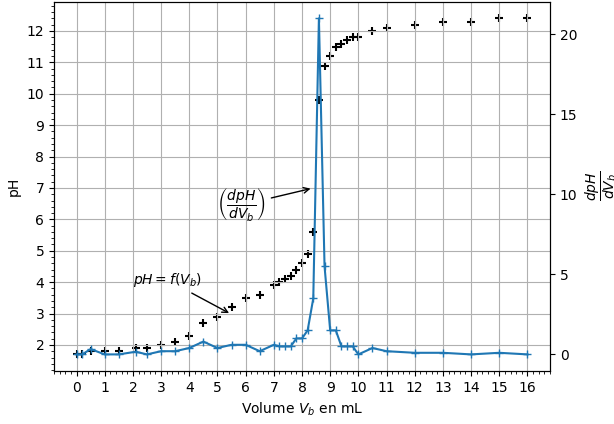
\includegraphics[scale = .7]{Ressources/TSPE_C8_Eval_Fig2.png}
    \caption{Représentation graphique du pH et $\dfrac{dpH}{dV_b}$ en fonction du volume de solution d'hydroxyde de sodium lors du titrage de l'acide oxalique par des ions hydroxyde}
    \label{fig:my_label}
\end{figure}\\
\textbf{Données : }\\
\begin{table}[h]
    \centering
    \begin{tabular}{|c|c|c|c|}
    \hline \textbf{Indicateur coloré} & \textbf{Couleur acide} & \textbf{Couleur basique} & \textbf{Zone de virage}\\
    \hline Bleu de bromothymol & jaune & bleu & 6,0 - 7,6\\
    \hline Rouge de crésol & jaune & rouge & 7,2 - 8,8\\
    \hline Phénolphtaléine & incolore & rose & 8,2 - 10\\
    \hline Héliantine & rouge & jaune & 3,1 - 4,4\\
    \hline
    \end{tabular}
    \caption{Liste d'indicateurs colorées et leurs zones de virage}
    \label{tab:my_label}
\end{table}
\begin{enumerate}
\setcounter{enumi}{4}
    \item Proposer le nom d'un indicateur coloré convenable, ainsi que le changement de couleur obtenu lors de l'équivalence si l'agent de laboratoire avait choisi un titrage colorimétrique.
    \item À l'aide de la figure 3, déterminer la concentration en quantité de matière en acide oxalique, puis justifier si le solide initial est dihydraté ou non. \emph{(Vous êtes invité à prendre des initiatives et à présenter la démarche suivie, même si elle n'a pas abouti.)}
\end{enumerate}
\end{document}